\section{Experiments}
\todo{Add 2 columns in Table 2}

We have implemented our method in python, utilising the NumPy \cite{numpy}
library for linear algebra operations and the SciPy \cite{scipy} library for an
implementation of \hcluster.
We have used a linkage-matrix \cite{scipy-hcluster-linkage}  based
data structure to store the tree, and have precomputed and cached several
operations that may need to be repeated every refinement iteration. This allows
us to quickly perform the merge and split operations and calculate the
scores, \todo{ ref earlier sections} without having to do (relatively)
expensive tree traversal operations in each iteration of the abstraction
refinement loop. 

Using this implementation, we have performed three sets of experiments to
demonstrate the usefulness of our technique. In several safety critical
settings, such as medical diagnosis and collision detection, where \dnn are
deployed as classifiers, false negative classification with respect to some
classes are highly undesirable. In the first set of experiments, we show that
our abstraction technique can be leverage to obtain effective compression of
\dnn in such settings with a guarantee that the compression does not introduce
any new false negative classifications (Section \ref{s:exp-mnist-comp}). In our
second set of experiments, we demonstrate how our technique may be used to
obtain abstract networks with the aim of proving a given property, plotting the
number of spurious counterexamples introduced as the size of the abstract
network reduces (Section \ref{s:exp-mnist-rob}). Finally, in the last set of
experiments, we show how our technique may be used in a CEGAR loop
\cite{cegar-nn} to verify the \acasxu properties.

\todo{TODO add gh link and exp machine details}

\subsection{Compression with Guarantees on Critical Classes}
\label{s:exp-mnist-comp}

In several safety-critical applications of \dnn as classifiers, there are
certain `critical` classes for which a false negative classification is far more
dangerous than a false positive one. For example, for medical diagnosis and
collision detection, a false negative is far more dangerous than a false
positive.

Safety critical analysis of neural networks is highly sensitive to the size of
the network. While several neural network compression techniques exist
\todo{cite}, they do not formal guarantees connecting the behavior
of the compressed network and the original network. Similarly, although existing
semantic abstraction techniques have been proposed as a way to compress neural
networks, the guarantees provided by such techniques are of an empirical nature
\cite{lin-comb-abs-jan}.
This lack of guarantees also limits the usefulness of these compression
techniques as optimisation steps when deploying a network to a
resource-constrained environment. 

Our theoretical framework for abstraction allows us to produce compressed
networks with the formal guarantee that the abstraction process will not
introduce any new false negative. We do this by marking the output neuron $n_c$
corresponding to the critical class in the output layer as inc, and all other
neurons in that layer as dec.  Then, for any input that the concrete network
classified into the critical class, $n_c$ will have the largest value in the
output layer, and as it has been marked as inc, it will continue to have the
larges value in the output layer for the abstract network as well. Thus, the
abstract network will also classify this input as critical. We will however pay
for this compression by introducing false positives, and in the subsequent plots
we plot the number of false positives introduced with respect to size of the
compressed network.

\begin{figure}
    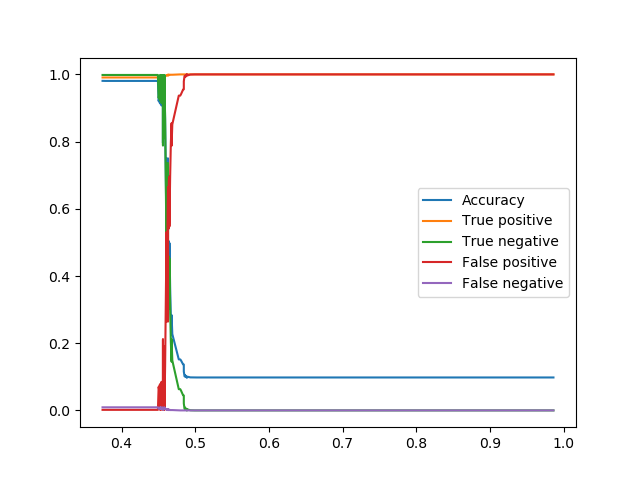
\includegraphics[scale=0.6]{figs/mnist_2_256_class_samples.png}
    \caption{Accuracy and True/False Positive/Negative Rates vs Reduction Rate
        plot for \mnist of size $2 \times 256$ with critical class 0. Refinement
    done via the 'samples' method. \todo{Shrink, add graph wrt no of steps}}
    \label{f:mnist-class-samples}
\end{figure}

We demonstrate the effectiveness of our abstraction method as such a compression
with guarantees technique via some experiments on \mnist and show the results in
figure \ref{f:mnist-class-samples}. We set the class '0'
as the critical class, and use our abstraction technique to obtain a compressed
network. Then, we use the 'samples' method described previously to progressively
refine the network (moving right to left) , plotting the accuracy, false/true
positive/negative rates as we go along. For this plot, the samples were drawn
from the \mnist training dataset, and the accuracies were plotted using the
\mnist test dataset.

We notice that, as guaranteed by the theory, the false negative rate never
increases, even as the reduction rate approaches close to $100\%$. Thus, even
for highly compressed networks, we never introduce any new false positives, and
in fact, the false negative rate improves, as some of the points that are going
to be newly classified as positive may in fact be true positives. However, as
discussed before, we do pay for the compression by introducing false positives,
which rises steeply in the graph. Thus, we see that a few refinement steps
contribute most to eliminating almost all of the false positives. 
This is similar to the behavior seen in Section \ref{s:exp-mnist-rob}, where a few
refinement steps leads to the elimination of most of the spurious
counterexamples all at once. 

We note that from the graph, even at around $45\%$ compression rate,
we find that the false positive rate is close to that of the original network.
This shows that our abstraction technique can find effective compressions with
the guarantee that no false negatives have been introduced. \todo{Add a table
smilar to later section for various mnist sizes?}

\subsection{Robustness on \mnist}
\label{s:exp-mnist-rob}
\todo{If time permits try: 1. These experiments on ACAS, 2. pgd then samples}

In this section, we start with our abstraction and progressively refine it using
our refinement technique, measuring the number of spurious counterexamples at
each step. To perform the refinement at each step, we try four methods to
perform the culprit neuron selection. The first method 'random' simply chooses a
culprit at random, and serves as a baseline. For the other three methods, we
choose a number of reference points to calculate scores, and choose the culprit
neuron with the highest score. For 'samples', the reference points are random
generated input points that satisfy the precondition. For 'pgd', the samples are
generated via a PGD \todo{cite} attack on the abstract network at each step. For
'samples-pgd', we do some initial refinement steps using the randomly generated
samples, when all the samples have been exhausted, we then perform 'pgd'. We use
the implementation of 'pgd' inside \abcrown for our experiments.

\begin{figure}
    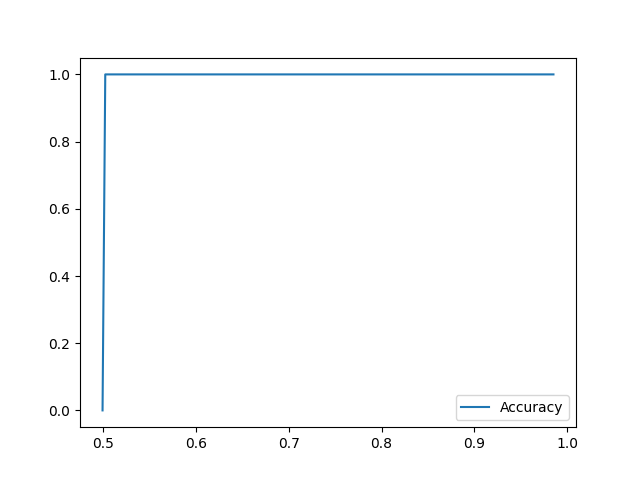
\includegraphics[scale=0.4]{figs/mnist_2_256_prop_0_0.03_samples.png}
    \caption{Accuracy vs Reduction Rate plot for \mnist of size $2 \times 256$
        with $\epsilon$-Robustness property. Refinement done via the 'samples'
    method.}
    \label{f:mnist-prop-samples}
\end{figure}
\begin{figure}
    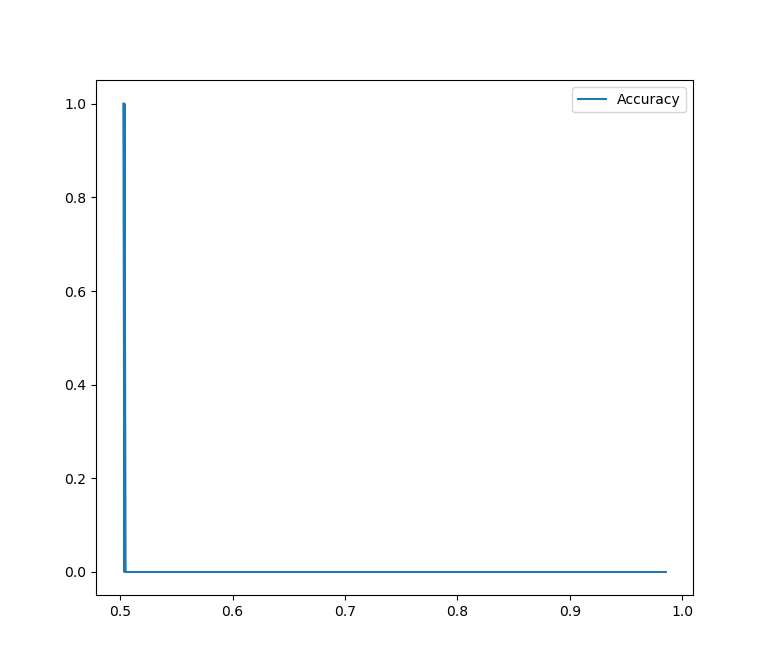
\includegraphics[scale=0.4]{figs/mnist_2_256_prop_0_0.03_pgd.png}
    \caption{Accuracy vs Reduction Rate plot for \mnist of size $2 \times 256$
        with $\epsilon$-Robustness property. Refinement done via the 'pgd'
    method.}
    \label{f:mnist-prop-pgd}
\end{figure}

Figure \ref{f:mnist-prop-samples} \ref{f:mnist-prop-pgd} shows a typical plot
for these experiments.  Here accuracy measures the number of true
counterexamples within a random sample
 We see that as we refine the
network and the reduction rate reduces (moving right to left along the graph),
the accuracy remains close to zero. At some point however, the accuracy jumps up
sharply and becomes close to $100\%$. This indicates that there are a few
critical refinement steps that remove almost all spurious counterexamples. This
may be due the fact that with epsilon robustness properties that are being
explored here, the pre-condition region may be very small, so a single
refinement step may change the behavior of the network on that small region in a
way that eliminates all possible spurious counterexamples from that region.
\todo{Make graphs smaller, and include the vs steps graphs}

\begin{table}
\begin{tabular}{|c|c|c|c|c|}
    \hline
    Net Size     & Cex Method  & Reduction & Accuracy & No. Steps \\
    \hline
    $2\times256$ & random      & $49.1\%$  & $100\%$  & $ 809$    \\
    $4\times256$ & random      & $49.6\%$  & $100\%$  & $1778$    \\
    $6\times256$ & random      & $49.7\%$  & $100\%$  & $2602$    \\
    $2\times256$ & samples     & $50.3\%$  & $100\%$  & $  27$    \\
    $4\times256$ & samples     & $49.9\%$  & $100\%$  & $ 648$    \\
    $6\times256$ & samples     & $47.9\%$  & $100\%$  & $1199$    \\
    $2\times256$ & pgd         & $50.4\%$  & $100\%$  & $  28$    \\
    $4\times256$ & pgd         & $88.6\%$  & $  0\%$  & $  14$    \\
    $6\times256$ & pgd         & $83.3\%$  & $  0\%$  & $  82$    \\
    $2\times256$ & samples-pgd & $50.3\%$  & $100\%$  & $  27$    \\
    $4\times256$ & samples-pgd & $49.9\%$  & $100\%$  & $ 648$    \\
    $6\times256$ & samples-pgd & $47.9\%$  & $100\%$  & $1209$    \\
    \hline
\end{tabular}
\caption{Summary of \mnist Results on a single robustness property \todo{Add
        column with time per refine, and number of neurons eliminated per
refine.}}
\label{t:mnist-prop-summary}
\end{table}

Table \ref{t:mnist-prop-summary} summarizes these results for multiple \mnist
networks and multiple refinement methods. Accuracy here refers to the final
accuracy of the best network found when the refinement process stops due to lack
of counterexamples. Firstly, we find that 'pgd' performs poorly on the $4$ and
$6$ layer networks, where while the number of steps are relatively low and the
reduction rate is high, the accuracy is very low. This is because the \abcrown
implementation of \pgd fails to find a spurious counterexample early on in the
refinement process for these instances, leading to early termination without
ever hitting the accuracy jump. 

Apart from these exceptions, the other instances and methods seem to perform
comparably on the same network in terms of reduction rate. This is evidence for
the fact that, within the limited search space of abstractions defined by our
tree, there exists a strong enough abstract network with a good reduction rate,
and that it is possible to find this network via a \cegar-like approach. 

Further, we see significant difference in the number of steps taken by 'random'
and the other methods in finding the abstract network. This indicates that our
heuristics for finding a culprit neuron to base the refinement on indeed
shortens the search for the refined network. We also observe that
'samples','samples-pgd' and for the $2$ layer network 'pgd' take similar number
of refinement steps, indicating that each method may be taking close to the
optimal set of refinement steps. So, although the 'pgd' method
incurs a significant time overhead \dmcmt{Measure?} it does not necessarily
provide any benefits. 

We note that in \cite{cleverest-nn}, an eager pgd-attack before each solver call
has been effectively used to accelerate the CEGAR loop. We do not see such
benefits from using pgd, and instead observe that the global view given by
the large number of samples in the `samples` method performs better. While the
relative performance of `pgd` and `samples` may be different for a different set
of target network and property, our framework allows the use of either, and
in-fact, any other method for generating the counterexamples.

\subsection{Verification of \acasxu}
\todo{These set of experiments still needs to be rerun}

In these set of experiments, we have taken the \acasxu set of
networks \todo{add detailed table} and
properties and attempt to verify them using a \cegar approach. We use our
technique to generate the abstraction, and attempt to verify the property on the
abstract network using an existing neural network verification solver. If the
solver returns a counterexample, and if that counterexample is not spurious, we
use that counterexample as a reference point for score calculation  to select
the culprit neuron (\ref{s:refinement}). With the culprit neuron selected, we
then refine the network.

\begin{table}
\begin{tabular}{ |c|c|c|c| }
\hline
Benchmarks &    \% Verified &  Avg Reduction &  Avg Time \\
\hline
safe       &        40.404  &         4.4875 &   14.198  \\
unsafe     &       100      &        55.6071 &   12.7916 \\
\hline
\end{tabular}
\caption{Summary of \acasxu Results \todo{Add full table in
appendix}}
\label{t:acas-summary}
\end{table}

The results are summarised in table \ref{t:acas-summary}. The solver we used was
\abcrown. The average times reported here do not include instances where the
verification failed due to timeout, and the reduction rate is with respect to
the network size after inc-dec split. We report these figures since, as noted in
\cite{cegar-nn}, the networks obtained after inc-dec split, while larger, are
easier to verify by typical solvers like \marabou.

We notice that for the unsafe cases, we are able to refute the
properties via a counterexample obtained on a significantly smaller network. In
fact, for most networks, we are able to refute based on a counterexample from
the fully abstracted network of size $18$ (See \todo{Add ref to full table in
appendix after re-runs}. Note that since we use only two classes in our
fully abstracted network as opposed to 4 in \cite{cegar-nn}, the size of this
network is significantly smaller. 

For safe cases, we see only negligible improvement in the size of the network.
We believe that this is because for these benchmarks, there is not much room for
improvement via abstraction. We are also able to only verify a smaller
percentage of these benchmarks, because the underlying solver call would time
out on mid-sized abstract networks \todo{Ref full table in appendix}, stalling
the CEGAR loop. We note that some timeouts were also reported in
\cite{cegar-nn}, and thus may be expected. 

In our experiments we find that the time taken for a solver call are more
dependent on the particular solver, solver configuration and benchmark than on
the size of the network. Thus it may seem that the effort needed to verify a
network is dependent on other factors than simply the size of the network. While
this may be interesting to explore in future work, we nonetheless argue that
network size is a relevant metric. This is as more and more solvers are designed
and optimized for various kinds of networks, the underlying worst case
performance will almost certainly remain exponential in the size of the network.
Furthermore, in the previous experiments (Sections \ref{s:exp-mnist-comp},
\ref{s:exp-mnist-rob}) we have demonstrated that our abstraction technique does
produce a reduction in network size whose usefulness extends beyond improving
verification time. 

